\documentclass[12pt]{article}
\usepackage[margin=0.7in]{geometry} 		% defines page margin
\usepackage{knitting} 				% defines \chart and \textknit
\usepackage{titling} 				% title page
\usepackage{graphicx,xspace, scrextend}	% defines space control stuff
\usepackage{tabularx, array, colortbl}	% defines tables
\usepackage{multicol} 				% defines columns
\usepackage{multirow} 				% defines multirows, combined cells in tables
\usepackage{framed, hyperref} 				% defines boxes for notes and written directions
\usepackage[x11names]{xcolor} 		% extends color library
\pdfmapfile{+knitfont.map}
\hypersetup{
    colorlinks=true,
    linkcolor=blue,
    filecolor=magenta,      
    urlcolor=blue,
}

% font selection
\usepackage{palatino, moresize, sectsty}
\allsectionsfont{\sffamily}

\renewcommand{\arraystretch}{2} % compresses tables for pattern keys

\newcolumntype{L}[1]{>{\leftalign\arraybackslash}p{#1}}
\newcolumntype{C}[1]{>{\centering\arraybackslash}p{#1}}

% length parameters
\setlength{\parindent}{0pt} % disables indentation for paragraphs
\setlength{\columnsep}{0.7cm} % column separation in multicol environment

% color parameters
\colorlet{framecolor}{black}
\colorlet{shadecolor}{LemonChiffon1}
\colorlet{highlight}{yellow}

% custom commands
\newcommand{\comment}[1]{} % allows for multiline comments that LaTeX will ignore

\newcommand{\vocab}[1]{\emph{\textbf{#1}}} % format for highlighting definitions of stitches, vocabulary terms
\newcommand{\rowDir}[1]{\textbf{#1:}} % indent for written instructions within paragraphs

\renewcommand{\repeat}[1]{\textbf{*[#1]*}} % format for written repeats, bold with *[ stitches ]*
\newcommand{\x}{$\times$}			% times symbol but shorthand
\newcommand{\setrepeat}[2]{\textbf{[#1]}\x{#2}}		% format for repeats with set number of repetitions, bold with [ stitches ]

\newcommand{\blank}{\underline{\hspace{2em}} } % written instructions, fill-in-the-blank box
\newcommand{\highlighted}[1]{\colorbox{highlight}{#1}} % written instructions, highlight particular text


% stitch count commands
\newcommand{\increase}[1]{(\emph{+#1 
	\ifnum#1=1{st}\else{sts}\fi})}
\newcommand{\decrease}[1]{(\emph{$-$#1
	\ifnum#1=1{st}\else{sts}\fi})}
\newcommand{\stitchcount}[1]{(\emph{#1 sts})}

% marker instructions
\renewcommand{\pm}[1]{\emph{pm #1}} % place stitch marker
\newcommand{\sm}{\emph{sm}} % slip marker
\renewcommand{\rm}[1]{\emph{rm #1}} % remove stitch marker

% thick horizontal line
\makeatletter \newcommand{\thickhline}{
    \noalign {\ifnum 0=`}\fi \hrule height 1.5pt
    \futurelet \reserved@a \@xhline
}
\makeatother

% custom environments
\newenvironment{frnote}
    {% framed environment for pattern notes
    	\setlength{\FrameRule}{1.5pt}
    	\def\FrameCommand{\fboxrule=\FrameRule\fboxsep=\FrameSep \fcolorbox{framecolor}{shadecolor}}
    	\MakeFramed {\FrameRestore}}
    {\setlength{\FrameRule}{1pt}
	\endMakeFramed}

\newenvironment{frdirection}
    {% framed environment for written directions
	\def\FrameCommand{\fboxrule=\FrameRule\fboxsep=\FrameSep \fbox}
   	\MakeFramed {\advance\hsize-\width \FrameRestore}
    	\addmargin[1.5cm]{0pt}}
    {\endaddmargin
	\endMakeFramed}

\newenvironment{unframed}
    {% unframed environment for written directions
	\begin{addmargin}[2em]{0pt}
	\setlength{\parindent}{-2em}
	}
    {%\vspace{1em}
	\setlength{\parindent}{0em}
	\end{addmargin}}

\title{Ifthen Socks} % pattern name here
\author{Shanel Wu (Piper Nell)}

\begin{document}

%%%%%%%%%%%%%%%%%%%%%%%%%%%%%%%%%%%%%%%%%%%%%%%%%%
% TITLE PAGE 
\begin{titlingpage}

% COVER PHOTO
% uncommend line below if you want a background fill image
% \ThisLRCornerWallPaper{1.0}{image.jpg} 

{\fontfamily{qag}\selectfont
\HUGE\textbf{\thetitle}
\hspace{4em} % adjust this space
\normalsize\theauthor
}


\begin{multicols}{2}
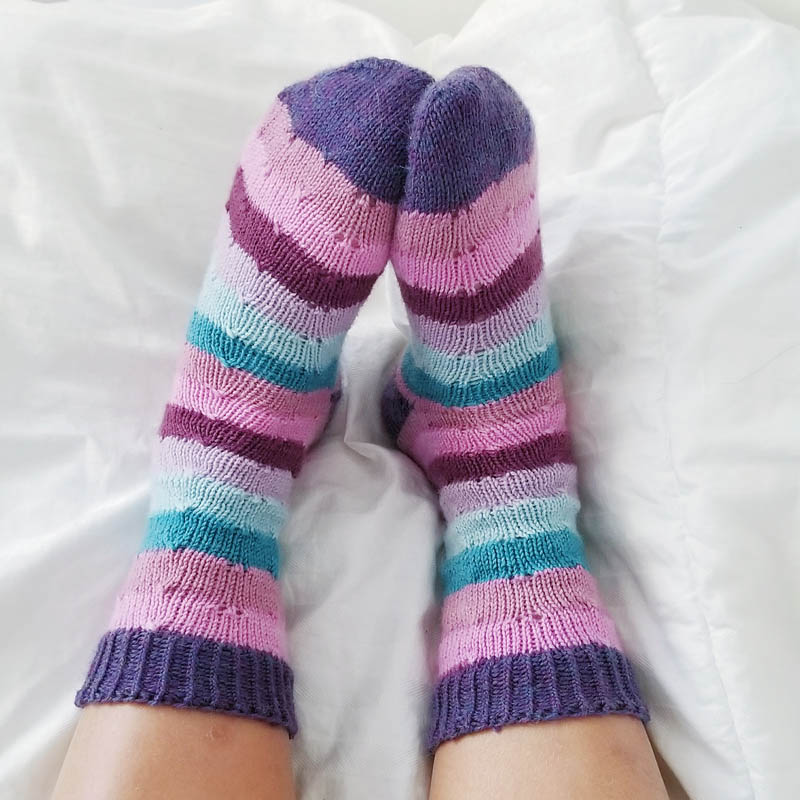
\includegraphics[width=0.9\linewidth]{bedtwo-small.jpg}
\vspace{1em}

% description
\textbf{IF} color change, \textbf{THEN} do this! That's all there is to this sock pattern for self-striping yarn.

\subsection*{Yarn Requirements}

% yardage, number of colors, etc.
You'll need 100g self-striping sock yarn in MC. Optionally, you'll also need 20g sock yarn in the same weight in CC.

\vspace{1em}

\emph{Sample used Knit Picks Felici in "Cheshire Grin" (100g/436y) as MC and Knit Picks Stroll in "Sprinkle Heather" (100g/462y) as CC.}

% also include: sample yarn, other yarn suggestions

\subsection*{Tools}

\begin{itemize}
\item Long circular needle for Magic Loop in your preferred size for socks 
\item Tapestry needle 
\end{itemize}

\subsection*{Sizing/Gauge}

% sample measurements, gauge, notes on ease, etc.

This pattern is written for three sock gauges: \vocab{S} (58 sts), \vocab{M} (66 sts), \vocab{L} (74 sts). Choose the stitch count that is closest to your normal sock gauge. Sample was knitted on 58 sts with US1/2.25mm needles.

\vfill
\columnbreak

\subsection*{Techniques}

Prior to knitting this pattern, you should be familiar with Magic Loop, Judy's Magic Cast On, basic lace techniques, and German short rows.

% discuss any special techniques and tutorials included


\subsection*{Pattern Key}

% formatting notes for charts and written directions
\vspace{-1em}
\small

% stitch key - fill in with all stitches used in design: chart symbol, written abbreviation, full stitch name or explanation
% stitches with explanations must first be BOLDED, followed by colon then explanation
\begin{center}
{\renewcommand{\arraystretch}{1.5}
\begin{tabular}{| C{0.2\linewidth}  p{0.7\linewidth} | }
\thickhline \rowcolor{shadecolor} 
 \textbf{Written}	& \textbf{Description} \\ \thickhline
k	&  knit \\
p	& purl   \\
st st 	& stockinette stitch \\
k tbl	& knit through the back loop \\
kfb	& \textbf{knit front back:} knit stitch through front loop as usual, then in the same stitch, knit through the back loop \\
m1l 		& \textbf{make 1 left:} with right needle, pick up bar between sts back to front, knit tbl \\
m1r 		& \textbf{make 1 right:} pick up bar between sts front to back, knit through front loop\\
s1		& \textbf{slip 1:} stitch purlwise with yarn in back (wyib) \\
yo		& yarn-over  \\
k2tog 	& knit 2 together \\
ssk		& slip slip knit \\
sk2p	& \textbf{slip k2tog psso:} slip 1 st knitwise, k2tog, pass slipped st over (psso)\\
double st &	\emph{See this linked tutorial for \href{http://asatricosa.com/german-short-rows/}{\underline{German Short Rows.}}}  \\
\hline
\end{tabular}
} 
\normalsize

\vspace{1em}
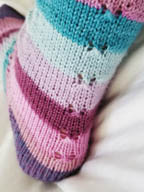
\includegraphics[height=0.5\linewidth]{backleg-small.jpg} \hspace{1em}
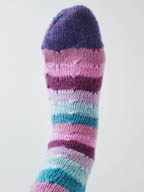
\includegraphics[height=0.5\linewidth]{frontfoot-small.jpg}
\end{center}
\end{multicols}
\end{titlingpage}

%%%%%%%%%%%%%%%%%%%%%%%%%%%%%%%%%%%%%%%%%%%%%%%%%%
% BEGIN INSTRUCTIONS

\section*{Toe-Up Instructions}
\begin{multicols}{2}

\subsection*{Rounded Toe}

Instructions are given for needle 1 only. Repeat each round instruction twice---once on needle 1 and once on needle 2---to complete a round.
Using CC, CO 18 sts with Judy's Magic CO \\ (9 sts on each needle). Work the following rounds through Round 17 (25, 33):

\rowDir{Rnd 1} k1, kfb, k to last 2 sts on needle, kfb, k1 \stitchcount{22} \\
\rowDir{Rnd 2} k1, m1l, k to last st on needle, m1r, k1 \stitchcount{26} \\
\rowDir{Rnds 3-5} Repeat Rnd 2 three times \stitchcount{38} \\
\rowDir{Rnd 6} k across \\
\rowDir{Rnd 7} Repeat Rnd 2 \stitchcount{42} \\
\rowDir{Rnds 8-13} Repeat Rnds 6-7 three times \stitchcount{54 sts} \\
\rowDir{Rnds 14-16} k across \\
\rowDir{Rnd 17} Repeat Rnd 2 \stitchcount{58} \\
\rowDir{Rnds 18-25} Repeat Rnds 14-17 twice \stitchcount{66} \\
\rowDir{Rnds 26-33} Repeat Rnds 14-17 twice \stitchcount{74}

\vspace{1em}

Break CC. Your ``instep stitches" are now on needle 1 and your ``sole stitches" are on needle 2. You should have 29 (33, 37) sts on each needle.

\subsection*{Foot}

Instructions are given for needle 1 (instep) only. Work round instruction once across needle 1, then k across needle 2 (sole). Join MC. This counts as a color change, so work the following \textbf{Foot Color Transition Rounds} once:

\rowDir{Rnd 1} s2, k11(13, 15), s3, k11(13, 15), s2 \\
\rowDir{Rnd 2} k2tog, k5(6, 7), yo, k1, yo, k5(6, 7), sk2p, k5(6, 7), yo, k1, yo, k5(6, 7), ssk \\

Continue in st st until next color change then work Foot Color Transition Rounds 1 and 2. Repeat until foot is desired length (approximately 1.5 to 2 in short of total foot length), then begin the heel.

\vfill
\columnbreak

\begin{frnote} \small
If you decide to use your own toe method, start with an odd number of sts on each needle.
\end{frnote}

\vspace{-1.5em}

\subsection*{German Short Row Heel}

Feel free to substitute a toe-up heel method of your choice. Contrasting heel is optional.

Work across instep as established. Your sole stitches will now become the ``heel stitches". 

\subsubsection*{Part 1}
Without breaking MC, join CC. Work back and forth on needle 2 as follows:

\rowDir{Row 1} (RS) k to 1 st from end, double st \\
\rowDir{Row 2} (WS) p to 1 st from end, double st \\
\rowDir{Row 3} k to double st, double st \\
\rowDir{Row 4} p to double st, double st \\

Repeat Rows 3 and 4 until there are 9 (10, 11) double sts on each side of the heel.

\subsubsection*{Boomerang}

Work the following rows once.

\rowDir{Row 1} (RS) k to double st, work all double sts as they come until you are 1 st from end, double st \\
\rowDir{Row 2} (WS) p to double st, work all double sts as they come, double st \\

\subsubsection*{Part 2}

Continue to work back and forth.

\small
\rowDir{Row 1} (RS) k to 9 (10, 11) sts from end, double st \\
\rowDir{Row 2} (WS) p to 9 (10, 11) sts from end, double st \\
\rowDir{Row 3} k to double st, work double st, double st \\
\rowDir{Row 4} p to double st, work double st, double st \\

\normalsize
Repeat Rows 3 and 4 until your double st is the last st at the end of a WS row. You should be back to where you left MC. Break CC and pick up MC. K across all heel sts, working double sts as they come, to complete the heel.

\newpage

\subsection*{Leg}

Your instep stitches will now become the ``front stitches" on needle 1 and your heel stitches will now become the ``back stitches" on needle 2. Round instructions are given for both needles. Work in st st until the next color change. Work \textbf{Leg Color Transition Rounds} 1 and 2 once as follows:

\rowDir{Rnd 1, front} s2, k11(13, 15), s3, k11(13, 15), s2 \\
\rowDir{Rnd 1, back} k13(15, 17), s3, k13(15, 17) \\
\rowDir{Rnd 2, front}  k2tog, k5(6, 7), yo, k1, yo, k5(6, 7), sk2p, k5(6, 7), yo, k1, yo, k5(6, 7), ssk \\
\rowDir{Rnd 2, back} k13(15, 17), yo, sk2p, yo, k13(15, 17) \\

Continue as established until leg is desired length. Break MC.

\subsection*{Cuff}

Join CC. Knit one complete round, then work \\ \repeat{k1 tbl, p1} until cuff is desired length. Bind off loosely and/or with a stretchy method such as Jeny's Surprisingly Stretchy BO. Weave in all ends.

\vfill
\columnbreak

\begin{flushright}
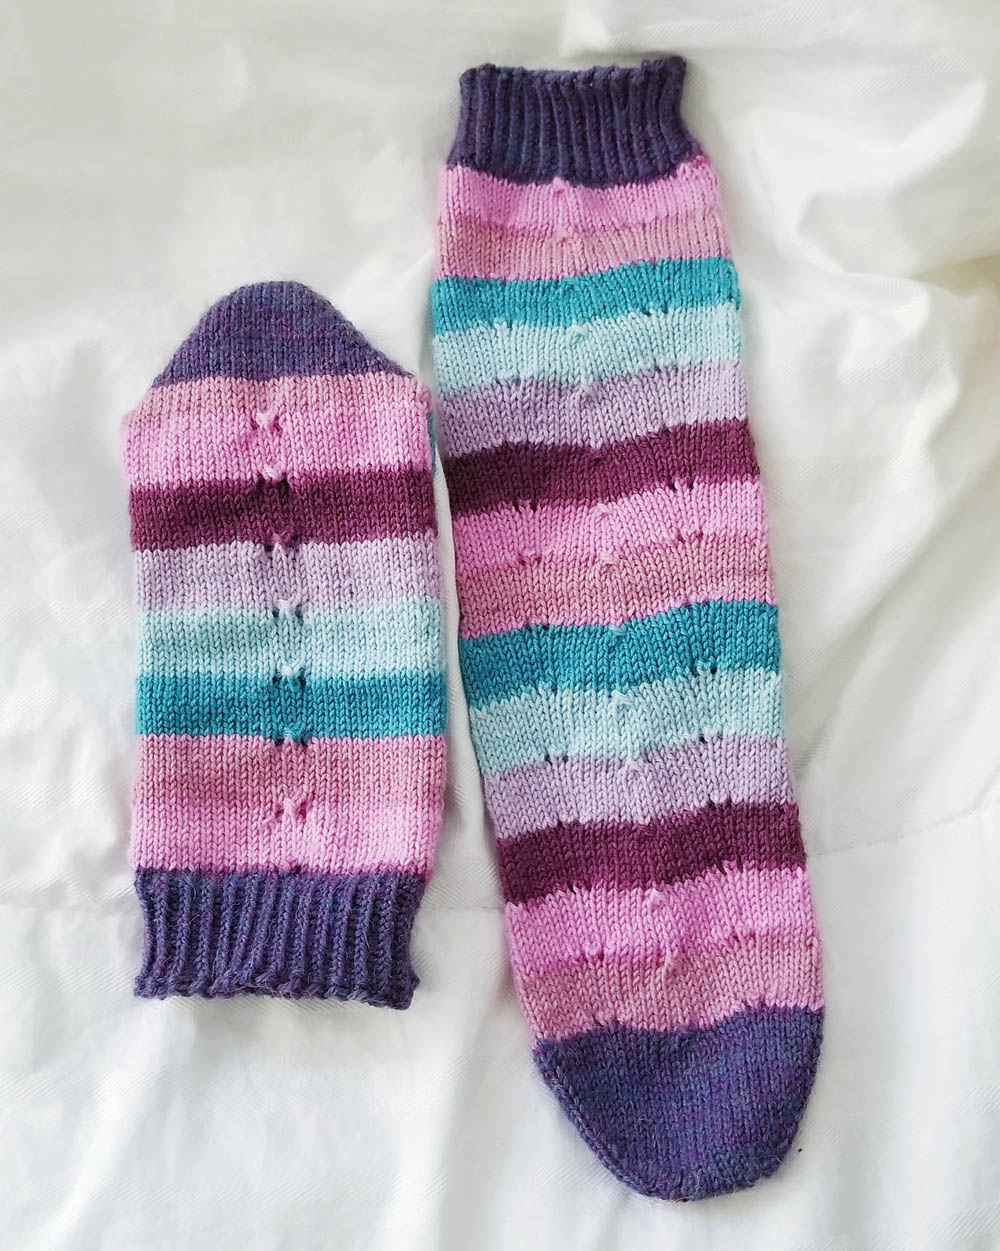
\includegraphics[width=0.9\linewidth]{laidflat-small.jpg}

\end{flushright}

\end{multicols}

\begin{frnote} \vspace{-1em}
\section*{Cuff Down Recipe}

These are not complete instructions for knitting the sock pattern cuff down. Rather, this is a recipe for adapting the pattern for cuff down socks. 

\vspace{1em}

\rowDir{Cuff} With CC, CO 58 (66, 74) sts. Work 1x1 twisted ribbing until cuff is desired length, then k one more round. Break CC.

\rowDir{Leg} Join MC. If you reach a color change, work the Leg Color Transition Rounds once. Otherwise, work st st. Continue until leg is desired length.

\rowDir{Heel} In CC, insert heel method of your choice. The German Short Row heel given in the toe-up instructions works here, too.

\rowDir{Foot} Rejoin MC. If you reach a color change, work the Foot Color Transition Rounds once. Otherwise, work st st. Continue until foot is desired length, about 2" short of total foot length. Break MC.

\rowDir{Toe} Join CC. Decrease and use kitchener stitch to graft toes together.

\end{frnote}

\vfill \ssmall
Pattern and photographs \copyright 2017 Shanel Wu. In downloading this free pattern, you agree to print and use this pattern only for personal use. Do not sell paper or electronic copies of this pattern.

%%%%%%%%%%%%%%%%%%%%%%%%%%%%%%%%%%%%%%%%%%%%%%%%%%
% APPENDICES (IF ANY)

\end{document}